% ----------------------------------------------------------------
% Os documentos e imagens adicionais da dissertação
% ----------------------------------------------------------------
\apendice

\chapter{Tabelas dos Valores Obtidos nos Testes}
\label{apendice_tabelas_valores}

As tabelas a seguir apresentam o Valor Obtido ($v_i$), o Valor Médio Acumulado ($VMA_i$) e a Variação de Valor Médio Acumulado ($Var_i$) em todas as métricas, para cada uma das execuções realizadas. As iterações encerram quando todas as métricas obtém Variação de Valor Médio Acumulado ($Var_i$) com valor igual ou inferior a 5\% (0.05) em duas iterações seguidas. O número mínimo de 5 execuções foi utilizado.

A Tabela abaixo é um modelo de representação das tabelas a seguir.

\begin{table}[htb]
\rowcolors{2}{gray!25}{white}
\centering
\resizebox{\textwidth}{!}{%
\begin{tabular}{ccllllll}
\rowcolor{gray!50}
\hline
\multicolumn{1}{c|}{Execução} & \multicolumn{1}{c|}{\begin{tabular}[c]{@{}c@{}}Nota de\\ Avaliação\\ Média\end{tabular}} & \multicolumn{1}{c|}{\begin{tabular}[c]{@{}c@{}}Dispersão\\ Média\end{tabular}} & \multicolumn{1}{c|}{\begin{tabular}[c]{@{}c@{}}Nota Local\\ Média\end{tabular}} & \multicolumn{1}{c|}{\begin{tabular}[c]{@{}c@{}}Nota Local\\ Máxima\end{tabular}} & \multicolumn{1}{c|}{$C_f$ Count} & \multicolumn{1}{c|}{\begin{tabular}[c]{@{}c@{}}Nota de\\ Avaliação\\ em $C_f$\end{tabular}} & \multicolumn{1}{c}{\begin{tabular}[c]{@{}c@{}}Dispersão\\ em $C_f$\end{tabular}} \\ \hline
\multicolumn{1}{c|}{} & \multicolumn{7}{c|}{Valores Obtido nesta Execução ($v$)} \\ \cline{2-8} 
\multicolumn{1}{c|}{} & \multicolumn{7}{c|}{Valores Médios Acumulados ($VMA$)} \\ \cline{2-8} 
\multicolumn{1}{c|}{\multirow{-3}{*}{1}} & \multicolumn{7}{c|}{Variação de Valor Médio Acumulado em relação à execução anterior ($Var$)} \\ \hline
\multicolumn{1}{c|}{...} & \multicolumn{1}{l|}{} & \multicolumn{1}{l|}{} & \multicolumn{1}{l|}{} & \multicolumn{1}{l|}{} & \multicolumn{1}{l|}{} & \multicolumn{1}{l|}{} &  \\ \hline
\multicolumn{1}{c|}{} & \multicolumn{7}{c|}{$v_i$} \\ \cline{2-8} 
\multicolumn{1}{c|}{} & \multicolumn{7}{c|}{${VMA}_i = (v_1 + v_2 + ... + v_{i-1} + v_i) / i$} \\ \cline{2-8} 
\multicolumn{1}{c|}{\multirow{-3}{*}{i}} & \multicolumn{7}{c|}{${Var}_i = ({VMA}_i / {VMA}_{i-1}) - 1$} \\ \hline
\multicolumn{1}{c|}{...} & \multicolumn{1}{r|}{} & \multicolumn{1}{r|}{} & \multicolumn{1}{r|}{} & \multicolumn{1}{r|}{} & \multicolumn{1}{r|}{} & \multicolumn{1}{r|}{} & \multicolumn{1}{r}{} \\ \hline
\multicolumn{1}{c|}{} & \multicolumn{7}{c|}{$v_{n-1}$} \\ \cline{2-8} 
\multicolumn{1}{c|}{} & \multicolumn{7}{c|}{${VMA}_{n-1}$} \\ \cline{2-8} 
\multicolumn{1}{c|}{\multirow{-3}{*}{n-1}} & \multicolumn{7}{c|}{\cellcolor[HTML]{ADDDAD}$|{Var}_{n-1}| \leq 0.05$} \\ \hline
\multicolumn{1}{c|}{} & \multicolumn{7}{c|}{$v_n$} \\ \cline{2-8} 
\multicolumn{1}{c|}{} & \multicolumn{7}{c|}{\cellcolor[HTML]{FFCE93}${VMA}_n$} \\ \cline{2-8} 
\multicolumn{1}{c|}{\multirow{-3}{*}{n}} & \multicolumn{7}{c|}{\cellcolor[HTML]{ADDDAD}$|{Var}_n| \leq 0.05$} \\ \hline 
\multicolumn{1}{l}{} & \multicolumn{1}{l}{} &  &  &  &  &  &  \\ \cline{2-4} \cline{6-8} 
\multicolumn{1}{l|}{\cellcolor[HTML]{FFFFFF}} & \multicolumn{3}{c|}{\cellcolor[HTML]{ADDDAD}Variação abaixo de 5\%} & \multicolumn{1}{l|}{\cellcolor[HTML]{FFFFFF}} & \multicolumn{3}{c|}{\cellcolor[HTML]{FFCE93}Valores utilizados} \\ \cline{2-4} \cline{6-8} 
\end{tabular}%
}
\end{table}

\pagebreak

\section{Algoritmo Genético}

Os valores de Nota de Avaliação em $C_f$ e Dispersão em $C_f$ não se aplicam à configuração \textbf{AG} conforme discutido na seção \ref{metricas}.

\begin{table}[!htb]
\rowcolors{2}{gray!25}{white}
\centering
\resizebox{\textwidth}{!}{%
\begin{tabular}{c|r|r|r|r|r|r|r}
\rowcolor{gray!50}
\hline
Execução & \multicolumn{1}{c|}{\begin{tabular}[c]{@{}c@{}}Nota de\\ Avaliação\\ Média\end{tabular}} & \multicolumn{1}{c|}{\begin{tabular}[c]{@{}c@{}}Dispersão\\ Média\end{tabular}} & \multicolumn{1}{c|}{\begin{tabular}[c]{@{}c@{}}Nota Local\\ Média\end{tabular}} & \multicolumn{1}{c|}{\begin{tabular}[c]{@{}c@{}}Nota Local\\ Máxima\end{tabular}} & \multicolumn{1}{c|}{$C_f$ Count} & \multicolumn{1}{c|}{\begin{tabular}[c]{@{}c@{}}Nota de\\ Avaliação\\ em $C_f$\end{tabular}} & \multicolumn{1}{c}{\begin{tabular}[c]{@{}c@{}}Dispersão\\ em $C_f$\end{tabular}} \\ \hline
 & 255.3900 & 43.0220 & 2.1450 & 15.0000 & 1.0000 & - & - \\ \cline{2-8} 
 & 255.3900 & 43.0220 & 2.1450 & 15.0000 & 1.0000 & - & - \\ \cline{2-8} 
\multirow{-3}{*}{1} & - & - & - & - & - & - & - \\ \hline
 & 292.3300 & 21.9953 & 0.5250 & 6.0000 & 0.0000 & - & - \\ \cline{2-8} 
 & 258.8600 & 32.5087 & 1.3350 & 10.5000 & 0.5000 & - & - \\ \cline{2-8} 
\multirow{-3}{*}{2} & 0.1485 & -0.2444 & -0.3776 & -0.3000 & -0.5000 & - & - \\ \hline
 & 263.7850 & 17.9270 & 0.8650 & 10.0000 & 0.0000 & - & - \\ \cline{2-8} 
 & 260.5017 & 27.6481 & 1.1783 & 10.3333 & 0.3333 & - & - \\ \cline{2-8} 
\multirow{-3}{*}{3} & \cellcolor[HTML]{ADDDAD}0.0063 & -0.1495 & -0.1174 & \cellcolor[HTML]{ADDDAD}-0.0159 & -0.3333 & - & - \\ \hline
 & 237.0050 & 28.4870 & 0.0750 & 15.0000 & 1.0000 & - & - \\ \cline{2-8} 
 & 254.6275 & 27.8578 & 0.9025 & 11.5000 & 0.5000 & - & - \\ \cline{2-8} 
\multirow{-3}{*}{4} & \cellcolor[HTML]{ADDDAD}-0.0225 & \cellcolor[HTML]{ADDDAD}0.0076 & -0.2341 & 0.1129 & 0.5000 & - & - \\ \hline
 & 260.0000 & 10.6010 & 0.0000 & 0.0000 & 0.0000 & - & - \\ \cline{2-8} 
 & 255.7020 & 24.4065 & 0.7220 & 9.2000 & 0.4000 & - & - \\ \cline{2-8} 
\multirow{-3}{*}{5} & \cellcolor[HTML]{ADDDAD}0.0042 & -0.1239 & -0.2000 & -0.2000 & -0.2000 & - & - \\ \hline
 & 241.0000 & 118.8943 & 0.0000 & 0.0000 & 0.0000 & - & - \\ \cline{2-8} 
 & 253.2517 & 40.1544 & 0.6017 & 7.6667 & 0.3333 & - & - \\ \cline{2-8} 
\multirow{-3}{*}{6} & \cellcolor[HTML]{ADDDAD}-0.0096 & 0.6452 & -0.1667 & -0.1667 & -0.1667 & - & - \\ \hline
 & 208.2350 & 40.6240 & 0.1500 & 15.0000 & 2.0000 & - & - \\ \cline{2-8} 
 & 246.8207 & 40.2215 & 0.5371 & 8.7143 & 0.5714 & - & - \\ \cline{2-8} 
\multirow{-3}{*}{7} & \cellcolor[HTML]{ADDDAD}-0.0254 & \cellcolor[HTML]{ADDDAD}0.0017 & -0.1072 & 0.1366 & 0.7143 & - & - \\ \hline
 & 226.1050 & 31.7023 & 0.2800 & 15.0000 & 1.0000 & - & - \\ \cline{2-8} 
 & 244.2313 & 39.1566 & 0.5050 & 9.5000 & 0.6250 & - & - \\ \cline{2-8} 
\multirow{-3}{*}{8} & \cellcolor[HTML]{ADDDAD}-0.0105 & \cellcolor[HTML]{ADDDAD}-0.0265 & -0.0598 & 0.0902 & 0.0938 & - & - \\ \hline
 & 277.3150 & 38.7190 & 0.7550 & 14.0000 & 0.0000 & - & - \\ \cline{2-8} 
 & 247.9072 & 39.1080 & 0.5328 & 10.0000 & 0.5556 & - & - \\ \cline{2-8} 
\multirow{-3}{*}{9} & \cellcolor[HTML]{ADDDAD}0.0151 & \cellcolor[HTML]{ADDDAD}-0.0012 & 0.0550 & 0.0526 & -0.1111 & - & - \\ \hline
 & 228.0000 & 29.9807 & 0.0000 & 0.0000 & 0.0000 & - & - \\ \cline{2-8} 
 & 245.9165 & 38.1953 & 0.4795 & 9.0000 & 0.5000 & - & - \\ \cline{2-8} 
\multirow{-3}{*}{10} & \cellcolor[HTML]{ADDDAD}-0.0080 & \cellcolor[HTML]{ADDDAD}-0.0233 & -0.1000 & -0.1000 & -0.1000 & - & - \\ \hline
 & 240.0050 & 29.3243 & 0.0750 & 15.0000 & 1.0000 & - & - \\ \cline{2-8} 
 & 245.3791 & 37.3888 & 0.4427 & 9.5455 & 0.5455 & - & - \\ \cline{2-8} 
\multirow{-3}{*}{11} & \cellcolor[HTML]{ADDDAD}-0.0022 & \cellcolor[HTML]{ADDDAD}-0.0211 & -0.0767 & 0.0606 & 0.0909 & - & - \\ \hline
 & 271.7650 & 62.5497 & 1.6800 & 15.0000 & 3.0000 & - & - \\ \cline{2-8} 
 & 247.5779 & 39.4865 & 0.5458 & 10.0000 & 0.7500 & - & - \\ \cline{2-8} 
\multirow{-3}{*}{12} & \cellcolor[HTML]{ADDDAD}0.0090 & 0.0561 & 0.2329 & \cellcolor[HTML]{ADDDAD}0.0476 & 0.3750 & - & - \\ \hline
 & 235.0000 & 17.3193 & 0.0000 & 0.0000 & 0.0000 & - & - \\ \cline{2-8} 
 & 246.6104 & 37.7805 & 0.5038 & 9.2308 & 0.6923 & - & - \\ \cline{2-8} 
\multirow{-3}{*}{13} & \cellcolor[HTML]{ADDDAD}-0.0039 & \cellcolor[HTML]{ADDDAD}-0.0432 & -0.0769 & -0.0769 & -0.0769 & - & - \\ \hline
 & 233.0050 & 10.1877 & 0.0750 & 15.0000 & 1.0000 & - & - \\ \cline{2-8} 
 & 245.6386 & 35.8095 & 0.4732 & 9.6429 & 0.7143 & - & - \\ \cline{2-8} 
\multirow{-3}{*}{14} & \cellcolor[HTML]{ADDDAD}-0.0039 & -0.0522 & -0.0608 & \cellcolor[HTML]{ADDDAD}0.0446 & \cellcolor[HTML]{ADDDAD}0.0317 & - & - \\ \hline
\end{tabular}%
}
\end{table}

\FloatBarrier
\pagebreak

\begin{table}[htb]
\rowcolors{2}{gray!25}{white}
\centering
\resizebox{\textwidth}{!}{%
\begin{tabular}{c|r|r|r|r|r|r|r}
\rowcolor{gray!50}
\hline
Execução & \multicolumn{1}{c|}{\begin{tabular}[c]{@{}c@{}}Nota de\\ Avaliação\\ Média\end{tabular}} & \multicolumn{1}{c|}{\begin{tabular}[c]{@{}c@{}}Dispersão\\ Média\end{tabular}} & \multicolumn{1}{c|}{\begin{tabular}[c]{@{}c@{}}Nota Local\\ Média\end{tabular}} & \multicolumn{1}{c|}{\begin{tabular}[c]{@{}c@{}}Nota Local\\ Máxima\end{tabular}} & \multicolumn{1}{c|}{$C_f$ Count} & \multicolumn{1}{c|}{\begin{tabular}[c]{@{}c@{}}Nota de\\ Avaliação\\ em $C_f$\end{tabular}} & \multicolumn{1}{c}{\begin{tabular}[c]{@{}c@{}}Dispersão\\ em $C_f$\end{tabular}} \\ \hline
 & 217.0000 & 48.4733 & 0.0000 & 0.0000 & 0.0000 & - & - \\ \cline{2-8} 
 & 243.7293 & 36.6538 & 0.4417 & 9.0000 & 0.6667 & - & - \\ \cline{2-8} 
\multirow{-3}{*}{15} & \cellcolor[HTML]{ADDDAD}-0.0078 & \cellcolor[HTML]{ADDDAD}0.0236 & -0.0667 & -0.0667 & -0.0667 & - & - \\ \hline
 & 232.0750 & 49.5183 & 0.3600 & 13.0000 & 0.0000 & - & - \\ \cline{2-8} 
 & 243.0009 & 37.4578 & 0.4366 & 9.2500 & 0.6250 & - & - \\ \cline{2-8} 
\multirow{-3}{*}{16} & \cellcolor[HTML]{ADDDAD}-0.0030 & \cellcolor[HTML]{ADDDAD}0.0219 & \cellcolor[HTML]{ADDDAD}-0.0116 & \cellcolor[HTML]{ADDDAD}0.0278 & -0.0625 & - & - \\ \hline
 & 256.0000 & 43.4033 & 0.0000 & 0.0000 & 0.0000 & - & - \\ \cline{2-8} 
 & 243.7656 & 37.8076 & 0.4109 & 8.7059 & 0.5882 & - & - \\ \cline{2-8} 
\multirow{-3}{*}{17} & \cellcolor[HTML]{ADDDAD}0.0031 & \cellcolor[HTML]{ADDDAD}0.0093 & -0.0588 & -0.0588 & -0.0588 & - & - \\ \hline
 & 227.0000 & 44.6817 & 0.0000 & 0.0000 & 0.0000 & - & - \\ \cline{2-8} 
 & 242.8342 & 38.1895 & 0.3881 & 8.2222 & 0.5556 & - & - \\ \cline{2-8} 
\multirow{-3}{*}{18} & \cellcolor[HTML]{ADDDAD}-0.0038 & \cellcolor[HTML]{ADDDAD}0.0101 & -0.0556 & -0.0556 & -0.0556 & - & - \\ \hline
 & 243.0300 & 10.6437 & 0.1950 & 13.0000 & 0.0000 & - & - \\ \cline{2-8} 
 & 242.8445 & 36.7397 & 0.3779 & 8.4737 & 0.5263 & - & - \\ \cline{2-8} 
\multirow{-3}{*}{19} & \cellcolor[HTML]{ADDDAD}0.0000 & \cellcolor[HTML]{ADDDAD}-0.0380 & \cellcolor[HTML]{ADDDAD}-0.0262 & \cellcolor[HTML]{ADDDAD}0.0306 & -0.0526 & - & - \\ \hline
 & 250.3850 & 37.5533 & 0.6100 & 14.0000 & 0.0000 & - & - \\ \cline{2-8} 
 & 243.2215 & 36.7804 & 0.3895 & 8.7500 & 0.5000 & - & - \\ \cline{2-8} 
\multirow{-3}{*}{20} & \cellcolor[HTML]{ADDDAD}0.0016 & \cellcolor[HTML]{ADDDAD}0.0011 & \cellcolor[HTML]{ADDDAD}0.0307 & \cellcolor[HTML]{ADDDAD}0.0326 & \cellcolor[HTML]{ADDDAD}-0.0500 & - & - \\ \hline
 & 247.0100 & 17.9377 & 0.1400 & 14.0000 & 0.0000 & - & - \\ \cline{2-8} 
 & \cellcolor[HTML]{FFCE93}243.4019 & \cellcolor[HTML]{FFCE93}35.8831 & \cellcolor[HTML]{FFCE93}0.3776 & \cellcolor[HTML]{FFCE93}9.0000 & \cellcolor[HTML]{FFCE93}0.4762 & - & - \\ \cline{2-8} 
\multirow{-3}{*}{21} & \cellcolor[HTML]{ADDDAD}0.0007 & \cellcolor[HTML]{ADDDAD}-0.0244 & \cellcolor[HTML]{ADDDAD}-0.0305 & \cellcolor[HTML]{ADDDAD}0.0286 & \cellcolor[HTML]{ADDDAD}-0.0476 & - & - \\ \hline
\end{tabular}%
}
\end{table}

Tempo total de execução: 875 segundos

\pagebreak
\section{Busca Inovativa}

\begin{table}[htb]
\rowcolors{2}{gray!25}{white}
\centering
\resizebox{\textwidth}{!}{%
\begin{tabular}{c|r|r|r|r|r|r|r}
\rowcolor{gray!50}
\hline
Execução & \multicolumn{1}{c|}{\begin{tabular}[c]{@{}c@{}}Nota de\\ Avaliação\\ Média\end{tabular}} & \multicolumn{1}{c|}{\begin{tabular}[c]{@{}c@{}}Dispersão\\ Média\end{tabular}} & \multicolumn{1}{c|}{\begin{tabular}[c]{@{}c@{}}Nota Local\\ Média\end{tabular}} & \multicolumn{1}{c|}{\begin{tabular}[c]{@{}c@{}}Nota Local\\ Máxima\end{tabular}} & \multicolumn{1}{c|}{$C_f$ Count} & \multicolumn{1}{c|}{\begin{tabular}[c]{@{}c@{}}Nota de\\ Avaliação\\ em $C_f$\end{tabular}} & \multicolumn{1}{c}{\begin{tabular}[c]{@{}c@{}}Dispersão\\ em $C_f$\end{tabular}} \\ \hline
 & 55.7400 & 1695.3943 & 7.9950 & 15.0000 & 14.0000 & 90.6429 & 2028.8901 \\ \cline{2-8} 
 & 55.7400 & 1695.3943 & 7.9950 & 15.0000 & 14.0000 & 90.6429 & 2028.8901 \\ \cline{2-8} 
\multirow{-3}{*}{1} & - & - & - & - & - & - & - \\ \hline
 & 74.2200 & 1692.8953 & 8.1450 & 15.0000 & 14.0000 & 105.1429 & 2032.7143 \\ \cline{2-8} 
 & 64.9800 & 1694.1448 & 8.0700 & 15.0000 & 14.0000 & 97.8929 & 2030.8022 \\ \cline{2-8} 
\multirow{-3}{*}{2} & 0.1658 & \cellcolor[HTML]{ADDDAD}-0.0007 & \cellcolor[HTML]{ADDDAD}0.0094 & \cellcolor[HTML]{ADDDAD}0.0000 & \cellcolor[HTML]{ADDDAD}0.0000 & 0.0800 & \cellcolor[HTML]{ADDDAD}0.0009 \\ \hline
 & 62.9100 & 1702.1457 & 7.7950 & 15.0000 & 11.0000 & 109.1818 & 2053.8182 \\ \cline{2-8} 
 & 64.2900 & 1696.8118 & 7.9783 & 15.0000 & 13.0000 & 101.6558 & 2038.4742 \\ \cline{2-8} 
\multirow{-3}{*}{3} & \cellcolor[HTML]{ADDDAD}-0.0106 & \cellcolor[HTML]{ADDDAD}0.0016 & \cellcolor[HTML]{ADDDAD}-0.0114 & \cellcolor[HTML]{ADDDAD}0.0000 & -0.0714 & \cellcolor[HTML]{ADDDAD}0.0384 & \cellcolor[HTML]{ADDDAD}0.0038 \\ \hline
 & 55.1800 & 1679.0587 & 7.7450 & 15.0000 & 8.0000 & 106.1250 & 2051.1429 \\ \cline{2-8} 
 & 62.0125 & 1692.3735 & 7.9200 & 15.0000 & 11.7500 & 102.7731 & 2041.6414 \\ \cline{2-8} 
\multirow{-3}{*}{4} & \cellcolor[HTML]{ADDDAD}-0.0354 & \cellcolor[HTML]{ADDDAD}-0.0026 & \cellcolor[HTML]{ADDDAD}-0.0073 & \cellcolor[HTML]{ADDDAD}0.0000 & -0.0962 & \cellcolor[HTML]{ADDDAD}0.0110 & \cellcolor[HTML]{ADDDAD}0.0016 \\ \hline
 & 65.0550 & 1697.0447 & 7.5400 & 15.0000 & 10.0000 & 103.1000 & 2049.3778 \\ \cline{2-8} 
 & 62.6210 & 1693.3077 & 7.8440 & 15.0000 & 11.4000 & 102.8385 & 2043.1886 \\ \cline{2-8} 
\multirow{-3}{*}{5} & \cellcolor[HTML]{ADDDAD}0.0098 & \cellcolor[HTML]{ADDDAD}0.0006 & \cellcolor[HTML]{ADDDAD}-0.0096 & \cellcolor[HTML]{ADDDAD}0.0000 & \cellcolor[HTML]{ADDDAD}-0.0298 & \cellcolor[HTML]{ADDDAD}0.0006 & \cellcolor[HTML]{ADDDAD}0.0008 \\ \hline
 & 70.8900 & 1691.3567 & 8.4750 & 15.0000 & 15.0000 & 104.0000 & 2041.7905 \\ \cline{2-8} 
 & 63.9992 & 1692.9826 & 7.9492 & 15.0000 & 12.0000 & 103.0321 & 2042.9556 \\ \cline{2-8} 
\multirow{-3}{*}{6} & \cellcolor[HTML]{ADDDAD}0.0220 & \cellcolor[HTML]{ADDDAD}-0.0002 & \cellcolor[HTML]{ADDDAD}0.0134 & \cellcolor[HTML]{ADDDAD}0.0000 & 0.0526 & \cellcolor[HTML]{ADDDAD}0.0019 & \cellcolor[HTML]{ADDDAD}-0.0001 \\ \hline
 & 52.7400 & 1685.8547 & 7.9600 & 15.0000 & 11.0000 & 88.4545 & 2050.5636 \\ \cline{2-8} 
 & 62.3907 & 1691.9643 & 7.9507 & 15.0000 & 11.8571 & 100.9496 & 2044.0425 \\ \cline{2-8} 
\multirow{-3}{*}{7} & \cellcolor[HTML]{ADDDAD}-0.0251 & \cellcolor[HTML]{ADDDAD}-0.0006 & \cellcolor[HTML]{ADDDAD}0.0002 & \cellcolor[HTML]{ADDDAD}0.0000 & \cellcolor[HTML]{ADDDAD}-0.0119 & \cellcolor[HTML]{ADDDAD}-0.0202 & \cellcolor[HTML]{ADDDAD}0.0005 \\ \hline
 & 67.2900 & 1692.4190 & 7.6050 & 15.0000 & 15.0000 & 99.7333 & 2049.5143 \\ \cline{2-8} 
 & \cellcolor[HTML]{FFCE93}63.0031 & \cellcolor[HTML]{FFCE93}1692.0211 & \cellcolor[HTML]{FFCE93}7.9075 & \cellcolor[HTML]{FFCE93}15.0000 & \cellcolor[HTML]{FFCE93}12.2500 & \cellcolor[HTML]{FFCE93}100.7976 & \cellcolor[HTML]{FFCE93}2044.7265 \\ \cline{2-8} 
\multirow{-3}{*}{8} & \cellcolor[HTML]{ADDDAD}0.0098 & \cellcolor[HTML]{ADDDAD}0.0000 & \cellcolor[HTML]{ADDDAD}-0.0054 & \cellcolor[HTML]{ADDDAD}0.0000 & \cellcolor[HTML]{ADDDAD}0.0331 & \cellcolor[HTML]{ADDDAD}-0.0015 & \cellcolor[HTML]{ADDDAD}0.0003 \\ \hline
\end{tabular}%
}
\end{table}

Tempo total de execução: 1634 segundos

\pagebreak
\section{Competição Local}

\begin{table}[htb]
\rowcolors{2}{gray!25}{white}
\centering
\resizebox{\textwidth}{!}{%
\begin{tabular}{c|r|r|r|r|r|r|r}
\rowcolor{gray!50}
\hline
Execução & \multicolumn{1}{c|}{\begin{tabular}[c]{@{}c@{}}Nota de\\ Avaliação\\ Média\end{tabular}} & \multicolumn{1}{c|}{\begin{tabular}[c]{@{}c@{}}Dispersão\\ Média\end{tabular}} & \multicolumn{1}{c|}{\begin{tabular}[c]{@{}c@{}}Nota Local\\ Média\end{tabular}} & \multicolumn{1}{c|}{\begin{tabular}[c]{@{}c@{}}Nota Local\\ Máxima\end{tabular}} & \multicolumn{1}{c|}{$C_f$ Count} & \multicolumn{1}{c|}{\begin{tabular}[c]{@{}c@{}}Nota de\\ Avaliação\\ em $C_f$\end{tabular}} & \multicolumn{1}{c}{\begin{tabular}[c]{@{}c@{}}Dispersão\\ em $C_f$\end{tabular}} \\ \hline
 & 102.0000 & 1675.3643 & 9.9100 & 15.0000 & 25.0000 & 129.6400 & 2037.5533 \\ \cline{2-8} 
 & 102.0000 & 1675.3643 & 9.9100 & 15.0000 & 25.0000 & 129.6400 & 2037.5533 \\ \cline{2-8} 
\multirow{-3}{*}{1} & - & - & - & - & - & - & - \\ \hline
 & 100.2050 & 1679.6123 & 9.3900 & 15.0000 & 22.0000 & 139.5455 & 2028.9134 \\ \cline{2-8} 
 & 101.1025 & 1677.4883 & 9.6500 & 15.0000 & 23.5000 & 134.5927 & 2033.2334 \\ \cline{2-8} 
\multirow{-3}{*}{2} & \cellcolor[HTML]{ADDDAD}-0.0088 & \cellcolor[HTML]{ADDDAD}0.0013 & \cellcolor[HTML]{ADDDAD}-0.0262 & \cellcolor[HTML]{ADDDAD}0.0000 & -0.0600 & \cellcolor[HTML]{ADDDAD}0.0382 & \cellcolor[HTML]{ADDDAD}-0.0021 \\ \hline
 & 103.5150 & 1683.0843 & 9.7500 & 15.0000 & 16.0000 & 129.1250 & 2050.2750 \\ \cline{2-8} 
 & 101.9067 & 1679.3537 & 9.6833 & 15.0000 & 21.0000 & 132.7702 & 2038.9139 \\ \cline{2-8} 
\multirow{-3}{*}{3} & \cellcolor[HTML]{ADDDAD}0.0080 & \cellcolor[HTML]{ADDDAD}0.0011 & \cellcolor[HTML]{ADDDAD}0.0035 & \cellcolor[HTML]{ADDDAD}0.0000 & -0.1064 & \cellcolor[HTML]{ADDDAD}-0.0135 & \cellcolor[HTML]{ADDDAD}0.0028 \\ \hline
 & 101.5450 & 1684.4330 & 9.5450 & 15.0000 & 24.0000 & 137.5833 & 2027.3949 \\ \cline{2-8} 
 & 101.8163 & 1680.6235 & 9.6488 & 15.0000 & 21.7500 & 133.9734 & 2036.0342 \\ \cline{2-8} 
\multirow{-3}{*}{4} & \cellcolor[HTML]{ADDDAD}-0.0009 & \cellcolor[HTML]{ADDDAD}0.0008 & \cellcolor[HTML]{ADDDAD}-0.0036 & \cellcolor[HTML]{ADDDAD}0.0000 & \cellcolor[HTML]{ADDDAD}0.0357 & \cellcolor[HTML]{ADDDAD}0.0091 & \cellcolor[HTML]{ADDDAD}-0.0014 \\ \hline
 & 103.9450 & 1687.1173 & 9.5750 & 15.0000 & 26.0000 & 134.7308 & 2029.9354 \\ \cline{2-8} 
 & \cellcolor[HTML]{FFCE93}102.2420 & \cellcolor[HTML]{FFCE93}1681.9223 & \cellcolor[HTML]{FFCE93}9.6340 & \cellcolor[HTML]{FFCE93}15.0000 & \cellcolor[HTML]{FFCE93}22.6000 & \cellcolor[HTML]{FFCE93}134.1249 & \cellcolor[HTML]{FFCE93}2034.8144 \\ \cline{2-8} 
\multirow{-3}{*}{5} & \cellcolor[HTML]{ADDDAD}0.0042 & \cellcolor[HTML]{ADDDAD}0.0008 & \cellcolor[HTML]{ADDDAD}-0.0150 & \cellcolor[HTML]{ADDDAD}0.0000 & \cellcolor[HTML]{ADDDAD}0.0391 & \cellcolor[HTML]{ADDDAD}0.0011 & \cellcolor[HTML]{ADDDAD}-0.0006 \\ \hline
\end{tabular}%
}
\end{table}

Tempo total de execução: 1008 segundos

\pagebreak
\section{Proposta}

\begin{table}[htb]
\rowcolors{2}{gray!25}{white}
\centering
\resizebox{\textwidth}{!}{%
\begin{tabular}{c|r|r|r|r|r|r|r}
\rowcolor{gray!50}
\hline
Execução & \multicolumn{1}{c|}{\begin{tabular}[c]{@{}c@{}}Nota de\\ Avaliação\\ Média\end{tabular}} & \multicolumn{1}{c|}{\begin{tabular}[c]{@{}c@{}}Dispersão\\ Média\end{tabular}} & \multicolumn{1}{c|}{\begin{tabular}[c]{@{}c@{}}Nota Local\\ Média\end{tabular}} & \multicolumn{1}{c|}{\begin{tabular}[c]{@{}c@{}}Nota Local\\ Máxima\end{tabular}} & \multicolumn{1}{c|}{$C_f$ Count} & \multicolumn{1}{c|}{\begin{tabular}[c]{@{}c@{}}Nota de\\ Avaliação\\ em $C_f$\end{tabular}} & \multicolumn{1}{c}{\begin{tabular}[c]{@{}c@{}}Dispersão\\ em $C_f$\end{tabular}} \\ \hline
 & 131.5750 & 1595.9700 & 9.4700 & 15.0000 & 17.0000 & 158.5294 & 1971.8824 \\ \cline{2-8} 
 & 131.5750 & 1595.9700 & 9.4700 & 15.0000 & 17.0000 & 158.5294 & 1971.8824 \\ \cline{2-8} 
\multirow{-3}{*}{1} & - & - & - & - & - & - & - \\ \hline
 & 137.1000 & 1550.8537 & 9.5100 & 15.0000 & 18.0000 & 160.2222 & 1995.2614 \\ \cline{2-8} 
 & 134.3375 & 1573.4118 & 9.4900 & 15.0000 & 17.5000 & 159.3758 & 1983.5719 \\ \cline{2-8} 
\multirow{-3}{*}{2} & \cellcolor[HTML]{ADDDAD}0.0210 & \cellcolor[HTML]{ADDDAD}-0.0141 & \cellcolor[HTML]{ADDDAD}0.0021 & \cellcolor[HTML]{ADDDAD}0.0000 & \cellcolor[HTML]{ADDDAD}0.0294 & \cellcolor[HTML]{ADDDAD}0.0053 & \cellcolor[HTML]{ADDDAD}0.0059 \\ \hline
 & 118.1550 & 1516.6340 & 9.3250 & 15.0000 & 17.0000 & 150.0000 & 1963.6397 \\ \cline{2-8} 
 & 128.9433 & 1554.4859 & 9.4350 & 15.0000 & 17.3333 & 156.2505 & 1976.9278 \\ \cline{2-8} 
\multirow{-3}{*}{3} & \cellcolor[HTML]{ADDDAD}-0.0402 & \cellcolor[HTML]{ADDDAD}-0.0120 & \cellcolor[HTML]{ADDDAD}-0.0058 & \cellcolor[HTML]{ADDDAD}0.0000 & \cellcolor[HTML]{ADDDAD}-0.0095 & \cellcolor[HTML]{ADDDAD}-0.0196 & \cellcolor[HTML]{ADDDAD}-0.0033 \\ \hline
 & 137.3200 & 1550.7850 & 9.1450 & 15.0000 & 19.0000 & 164.7368 & 1987.4269 \\ \cline{2-8} 
 & 131.0375 & 1553.5607 & 9.3625 & 15.0000 & 17.7500 & 158.3721 & 1979.5526 \\ \cline{2-8} 
\multirow{-3}{*}{4} & \cellcolor[HTML]{ADDDAD}0.0162 & \cellcolor[HTML]{ADDDAD}-0.0006 & \cellcolor[HTML]{ADDDAD}-0.0077 & \cellcolor[HTML]{ADDDAD}0.0000 & \cellcolor[HTML]{ADDDAD}0.0240 & \cellcolor[HTML]{ADDDAD}0.0136 & \cellcolor[HTML]{ADDDAD}0.0013 \\ \hline
 & 135.9750 & 1562.5000 & 9.9100 & 15.0000 & 23.0000 & 156.4783 & 1923.7036 \\ \cline{2-8} 
 & 132.0250 & 1555.3485 & 9.4720 & 15.0000 & 18.8000 & 157.9933 & 1968.3828 \\ \cline{2-8} 
\multirow{-3}{*}{5} & \cellcolor[HTML]{ADDDAD}0.0075 & \cellcolor[HTML]{ADDDAD}0.0012 & \cellcolor[HTML]{ADDDAD}0.0117 & \cellcolor[HTML]{ADDDAD}0.0000 & 0.0592 & \cellcolor[HTML]{ADDDAD}-0.0024 & \cellcolor[HTML]{ADDDAD}-0.0056 \\ \hline
 & 137.9550 & 1506.9420 & 9.1050 & 15.0000 & 16.0000 & 162.9375 & 1971.1250 \\ \cline{2-8} 
 & 133.0133 & 1547.2808 & 9.4108 & 15.0000 & 18.3333 & 158.8174 & 1968.8398 \\ \cline{2-8} 
\multirow{-3}{*}{6} & \cellcolor[HTML]{ADDDAD}0.0075 & \cellcolor[HTML]{ADDDAD}-0.0052 & \cellcolor[HTML]{ADDDAD}-0.0065 & \cellcolor[HTML]{ADDDAD}0.0000 & \cellcolor[HTML]{ADDDAD}-0.0248 & \cellcolor[HTML]{ADDDAD}0.0052 & \cellcolor[HTML]{ADDDAD}0.0002 \\ \hline
 & 138.2950 & 1567.2277 & 9.7600 & 15.0000 & 19.0000 & 162.5263 & 1990.7251 \\ \cline{2-8} 
 & \cellcolor[HTML]{FFCE93}133.7679 & \cellcolor[HTML]{FFCE93}1550.1303 & \cellcolor[HTML]{FFCE93}9.4607 & \cellcolor[HTML]{FFCE93}15.0000 & \cellcolor[HTML]{FFCE93}18.4286 & \cellcolor[HTML]{FFCE93}159.3472 & \cellcolor[HTML]{FFCE93}1971.9663 \\ \cline{2-8} 
\multirow{-3}{*}{7} & \cellcolor[HTML]{ADDDAD}0.0057 & \cellcolor[HTML]{ADDDAD}0.0018 & \cellcolor[HTML]{ADDDAD}0.0053 & \cellcolor[HTML]{ADDDAD}0.0000 & \cellcolor[HTML]{ADDDAD}0.0052 & \cellcolor[HTML]{ADDDAD}0.0033 & \cellcolor[HTML]{ADDDAD}0.0016 \\ \hline
\end{tabular}%
}
\end{table}

Tempo total de execução: 1401 segundos

\chapter{Exemplos de Mapas Obtidos}
\label{exemplos_mapas}

\section{Algoritmo Genético}

Mapas contidos no conjunto $C_f$ da 12ª execução da configuração \textbf{AG}.

\begin{figure}[htb]
	\begin{center}
		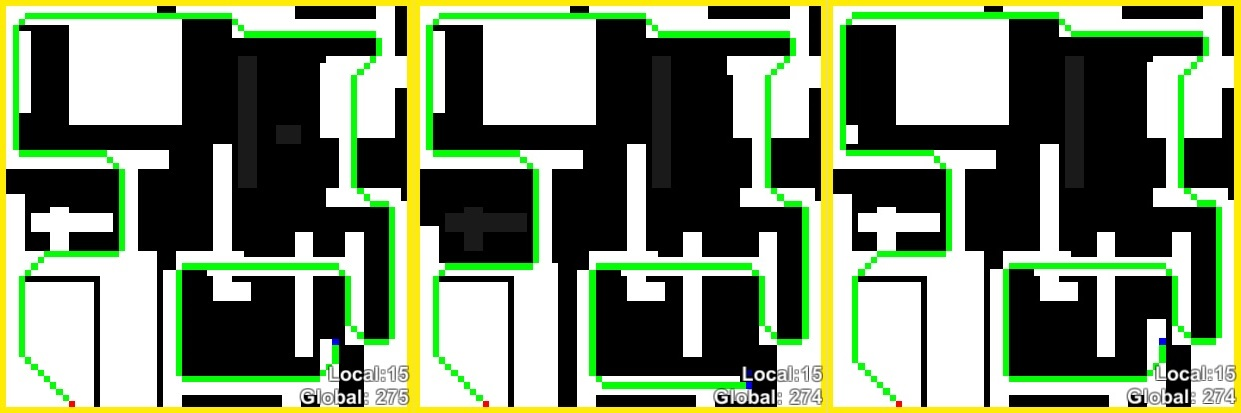
\includegraphics[width=1\textwidth]{Imagens/maps_ag.jpg}
	\end{center}
\end{figure}

\FloatBarrier
\pagebreak

\section{Busca Inovativa}

Mapas contidos no conjunto $C_f$ da 3ª execução da configuração \textbf{NS}.

\begin{figure}[htb]
	\begin{center}
		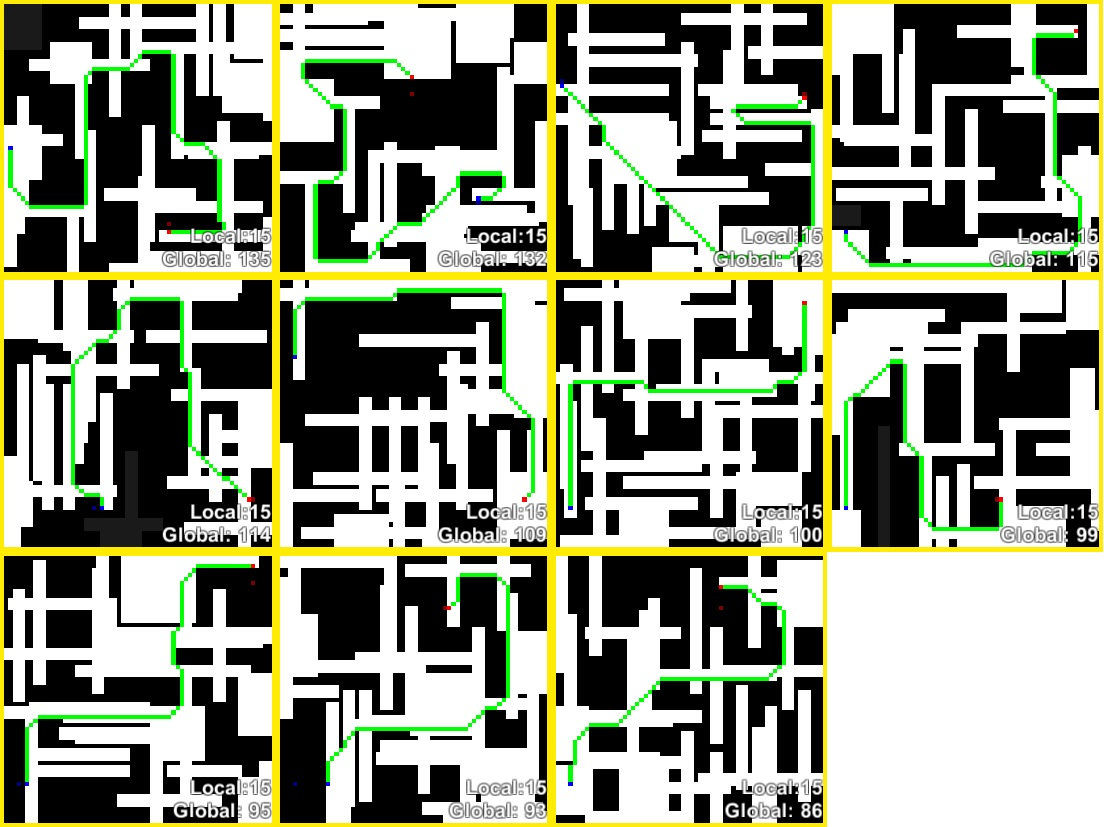
\includegraphics[width=1\textwidth]{Imagens/maps_ns.jpg}
	\end{center}
\end{figure}

\FloatBarrier
\pagebreak

\section{Competição Local}

Mapas contidos no conjunto $C_f$ da 3ª execução da configuração \textbf{Lehman}.

\begin{figure}[htb]
	\begin{center}
		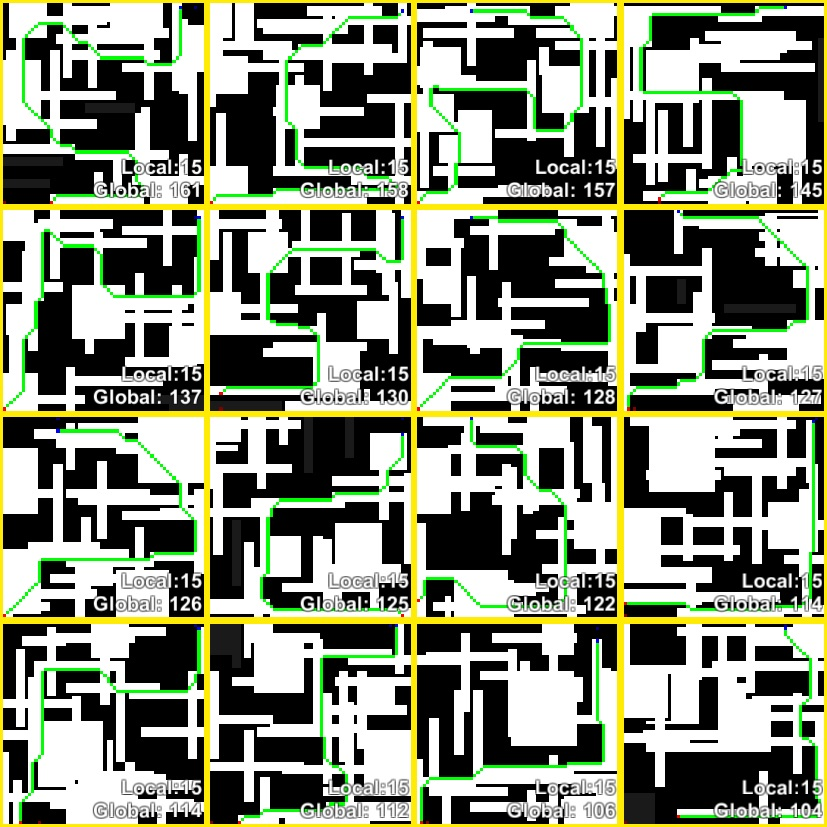
\includegraphics[width=1\textwidth]{Imagens/maps_lehman.jpg}
	\end{center}
\end{figure}

\FloatBarrier
\pagebreak

\section{Proposta}

Mapas contidos no conjunto $C_f$ da 6ª execução da configuração \textbf{Proposta}.

\begin{figure}[htb]
	\begin{center}
		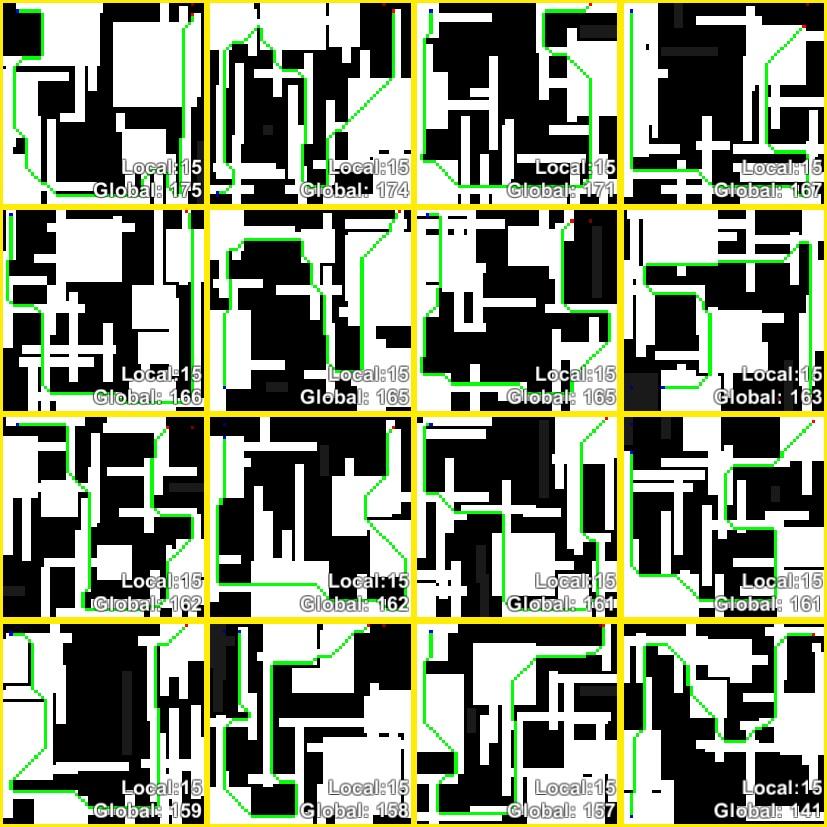
\includegraphics[width=1\textwidth]{Imagens/maps_melotti.jpg}
	\end{center}
\end{figure}

\FloatBarrier